\chapter{Plataforma de desarrollo}
\label{cap:capitulo4}

\begin{flushright}
\begin{minipage}[]{10cm}
\emph{El mundo no es sino un lienzo para nuestra imaginación.}\\
\end{minipage}\\

Henry David Thoreau\\
\end{flushright}

\vspace{1cm}

Tras definir los objetivos del proyecto, en este capítulo se presentan las plataformas de desarrollo, tanto \textit{hardware} como \textit{software}, utilizadas para alcanzarlos.


\section{Hardware}
\label{sec:hardware}

En esta sección se describen los componentes físicos que se han utilizado en el desarrollo del proyecto, prestando especial atención a su precio, priorizando piezas \textit{low-cost}, para la consecución del objetivo 3 descrito en la sección ~\ref{sec:Requisitos}.


\subsection{Raspberry Pi 4}

La Raspberry Pi\footnote{https://www.raspberrypi.com/products/raspberry-pi-4-model-b/} (Figura \ref{fig:raspberry}) es un microcomputador de propósito general, de bajo coste y tamaño reducido, muy útil para proyectos educativos, de electrónica y de robótica, como el presente proyecto.

\vspace{0.2cm}

\begin{figure} [h!]
  \begin{center}
    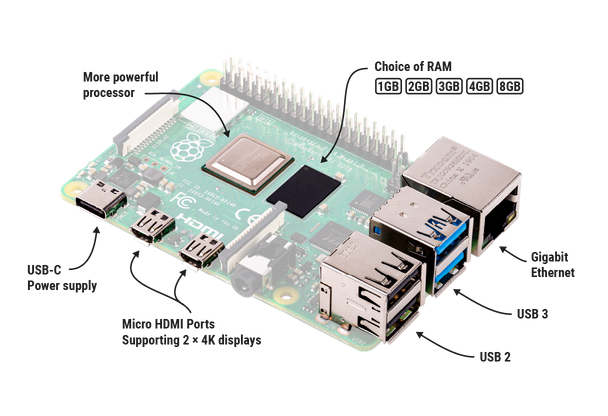
\includegraphics[width=11cm]{figs/raspberry}
  \end{center}
  \caption{\textit{Raspberry Pi 4}, Fundación Raspberry Pi}
  \label{fig:raspberry}
\end{figure}\


Cuenta con 40 pines GPIO (\textit{General Purpose Input/Output}) que permiten la conexión de diversos componentes, como motores, sensores o LED. Existen dos tipos de numeración para estos pines: BCM (\textit{Broadcom SOC channel}) y BOARD.

Los diferentes tipos de pines son:

\begin{itemize}
	\item \texttt{GND}: Se usa para cerrar el circuito eléctrico, asegurando un funcionamiento correcto y estable.
	Según la numeración BOARD, los pines GND son: 6, 9, 14, 20, 25, 30, 34 y 39.
	En el proyecto se han utilizado los siguientes pines: 39 para el pulsador, 25 para el LCD y 34 para el LED.

	\item \texttt{5V}: Se usa para alimentar a los componentes conectados directamente desde la placa con 5 voltios.
	Según la numeración BOARD, los pines 5V  son: 2 y 4.
    En el proyecto se ha utilizado el pin 2 para el ventilador de la placa.

	\item \texttt{3.3V}: Se usa para alimentar a los componentes conectados directamente desde la placa con 3.3 voltios.
	Según la numeración BOARD, los pines 3.3V son: 1 y 17.
	En el proyecto se ha utilizado el pin 1 para el LCD.

    \item \texttt{I2C (Inter-Integrated Circuit)}: Bus de comunicación que permite conectar la Raspberry con dispositivos externos.
    Los pines I2C de la placa, según la numeración BOARD son: 3 (SDA  \textit{Serial Data Line}) y 5 (SCL \textit{Serial Clock}).


    \item \texttt{SPI (Serial Peripheral Interface)}: Bus de comunicación serial de alta velocidad.
    Según la numeración BOARD, los pines SPI son: 19 (MOSI \textit{Master Output Slave Input}), 21 (MISO \textit{Master In Slave Out}), 23 (SCLK \textit{Serial Clock}), 24 (CE0 \textit{Chip Enable 0}) y 26 (CE1 \textit{Chip Enable 1}).
    En el proyecto se han utilizado los pines 19, 21, 23 para el LCD.

    \item \texttt{UART (Universal Asynchronous Receiver-Transmitter)}: Se usa para la comunicación serial entre la placa y otros dispositivos.
    Según la numeración BOARD, los pines UART son: 8 (TDX \textit{Transmitter}) y 10 (RDX \textit{Receiver}).

    \item \texttt{PWM (Pulse Width Modulation)}: Se usa para simular salidas analógicas usando pines digitales.
    Según la numeración BOARD, los pines PWM de la placa son: 12, 32, 33 y 35.

    \item \texttt{GPIO}: Pines de propósito general para entrada/salida digital.

\end{itemize}


Además, dispone de una ranura para tarjeta MicroSD, que permite la instalación de un sistema operativo y el almacenamiento de datos.


\subsection{Mini Cámara Web}

Para el reconocimiento facial del sistema, se ha utilizado una cámara web (Figura \ref{fig:camara})  externa de tipo USB. El dispositivo cuenta con un sensor CMOS (Semiconductor de óxido Metálico Complementario) de 2 megapíxeles, capaz de capturar vídeos en resolución Full HD (1920x1080) a una velocidad de hasta 30 fotogramas por segundo.

\vspace{0.2cm}

La cámara utiliza una interfaz 2.0 USB con soporte \textit{plug and play}, lo que permite su funcionamiento sin necesidad de instalar controladores adicionales.

\vspace{0.2cm}

El dispositivo presenta unas dimensiones de 70 mm x 50.7 mm x 44 mm y un peso aproximado de 62.8 gramos.


\begin{figure} [h!]
  \begin{center}
    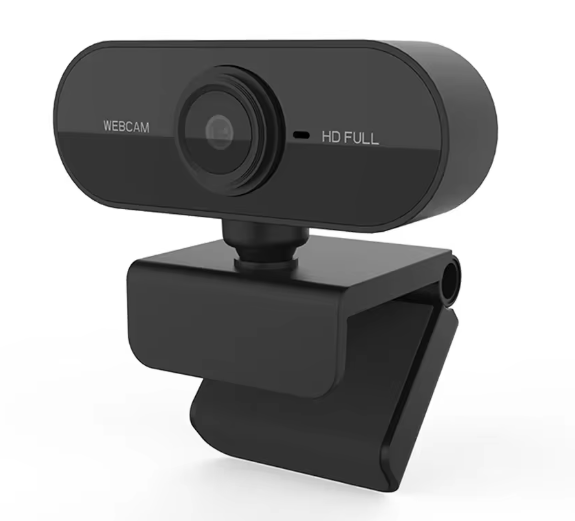
\includegraphics[width=6cm]{figs/camara}
  \end{center}
  \caption{Cámara web}
  \label{fig:camara}
\end{figure}\


\subsection{Pantalla táctil}

El sistema del proyecto cuenta con una interfaz gráfica que permite la interacción directa del usuario con el robot, ofreciendo funcionalidades como juegos de memoria, búsquedas básicas y otras actividades orientadas a la estimulación cognitiva.

\vspace{0.2cm}

Para la visualización e interacción con dicha interfaz, se ha utilizado una pantalla táctil (Figura \ref{fig:pantalla}) capacitiva de 10 pulgadas, equipada con altavoces integrados y compatible con la Raspberry Pi. La pantalla tiene una resolución de 1080x600 píxeles, lo que permite una visualización clara de la interfaz del robot.

\vspace{0.2cm}

La elección de esta pantalla se basó en sus dimensiones y resolución, que facilitan una visualización accesible y cómoda para personas mayores, mejorando la funcionalidad del sistema.

\vspace{0.2cm}

\begin{figure} [h!]
  \begin{center}
    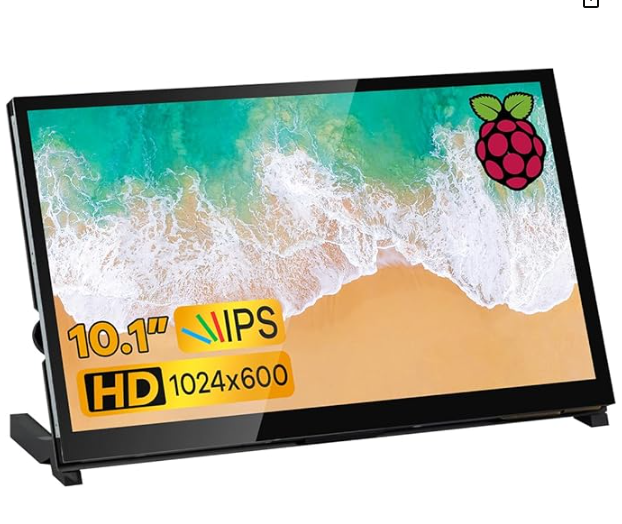
\includegraphics[width=7cm]{figs/pantalla}
  \end{center}
  \caption{LAFVIN Pantalla táctil }
  \label{fig:pantalla}
\end{figure}\


\subsection{Pantalla TFT (Thin Film Transistor )}

El módulo ILI9488 (Figura \ref{fig:lcd}), de 2.4 pulgadas, presenta unas dimensiones de 98 mm x 56mm y se alimenta con 3.3 V. Este tipo de pantalla permite el control individual de cada píxel, facilitando la representación de gráficos e imágenes.

\vspace{0.2cm}

A diferencia de los LCD convencionales, donde la visualización se limita a la  activación de segmentos predefinidos (generalmente en un solo color), las pantallas TFT como la mencionada emplean píxeles compuestos por tres canales (RGB: Red Green Blue), lo que permite obtener una amplia gama de colores. Gracias a ello, es posible realizar una interfaz más vistosas e intuitiva para el usuario.

\vspace{0.2cm}

Este módulo ha sido empleado en el proyecto para proporcionar retroalimentación visual al usuario mediante la representación de formas que simulan expresiones del robot, aportando así una mayor sensación de empatía. Además, se emplea para mostrar mensajes de estado con el objetivo de que el usuario comprenda el funcionamiento interno del sistema y evitar confusiones en su comportamiento.

\vspace{0.2cm}

\begin{figure} [h!]
  \begin{center}
    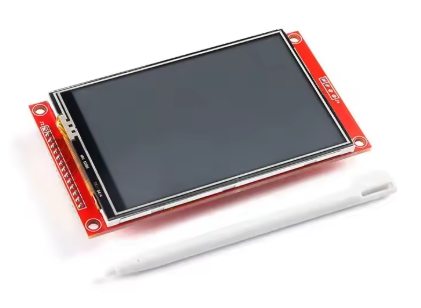
\includegraphics[width=5cm]{figs/lcd}
  \end{center}
  \caption{Módulo ILI9488}
  \label{fig:lcd}
\end{figure}\


\subsection{Micrófono USB}

Para capturar el audio se ha utilizado un micrófono de tipo lavalier con clip (Figura \ref{fig:micro}), caracterizado por su tamaño reducido y su fácil integración en el sistema.

\vspace{0.2cm}

Este micrófono es compatible con la Raspberry Pi mediante conexión USB, lo que facilita su instalación al no requerir hardware adicional.

\vspace{0.2cm}

La elección de este modelo se debe a su flexibilidad de colocación, una característica clave en este proyecto, ya que permite situar el micrófono cerca del usuario. Esto favorece el reconocimiento de comandos de voz y las interacciones con el sistema.


\vspace{0.2cm}

\begin{figure} [h!]
  \begin{center}
    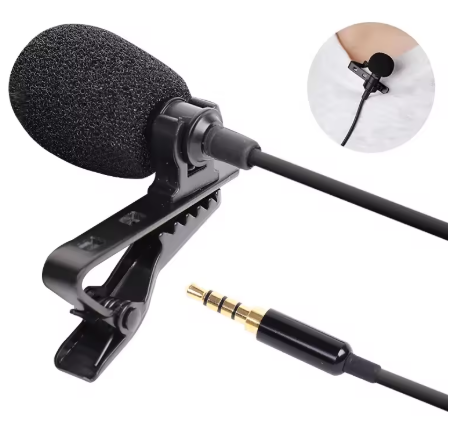
\includegraphics[width=4cm]{figs/micro}
  \end{center}
  \caption{Micrófono USB}
  \label{fig:micro}
\end{figure}\



\subsection{Multímetro}

Para comprobar el correcto funcionamiento de los componentes y sus conexiones se ha utilizado un multímetro (Figura \ref{fig:multi}). Este instrumento permite medir el voltaje, facilitando la verificación de la alimentación y la detección de fallos en el circuito electrónico.

\vspace{0.2cm}

Su uso ha resultado primordial durante el montaje y prueba del sistema, asegurando un correcto funcionamiento del mismo.

\vspace{0.2cm}

\begin{figure}[h!]
  \begin{center}
    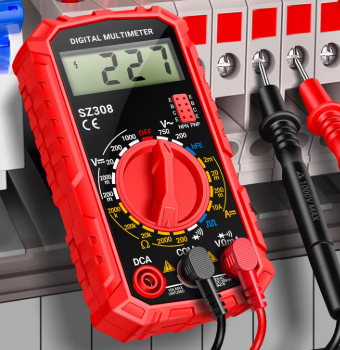
\includegraphics[width=5cm]{figs/multi}
  \end{center}
  \caption{ANENG-multímetro Digital SZ308}
  \label{fig:multi}
\end{figure}\


\subsection{Sensor de infrarrojo}

Con el objetivo de detectar desniveles en el entorno y prevenir caídas del robot, especialmente en zonas como mesas u otras superficies elevadas, se han utilizado dos sensores de infrarrojos (Figura \ref{fig:infra}).

Estos sensores permiten detectar la ausencia de superficie mediante la emisión y recepción de luz infrarroja.

\begin{figure} [h!]
  \begin{center}
    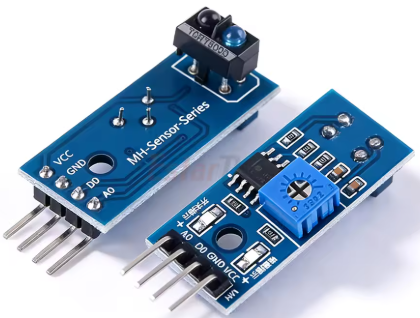
\includegraphics[width=4cm]{figs/infra}
  \end{center}
  \caption{Sensor infrarrojo reflectante TCRT5000}
  \label{fig:infra}
\end{figure}\


\subsection{Controlador L298N}

La Raspberry Pi no puede alimentar directamente los motores debido a las limitaciones de corriente de los pines GPIO. Por ese motivo, se hace uso de una placa controladora L298N (Figura \ref{fig:control}) para gestionar la alimentación y el control de los motores.

Este controlador permite accionar dos motores, con la posibilidad de controlar su velocidad y dirección. Además, puede ser alimentado con tensiones de hasta 26V.

En el siguiente Cuadro \ref{cuadro:control} se encuentran las principales especificaciones del controlador.


\vspace{0.2cm}


\begin{figure} [h!]
  \begin{center}
    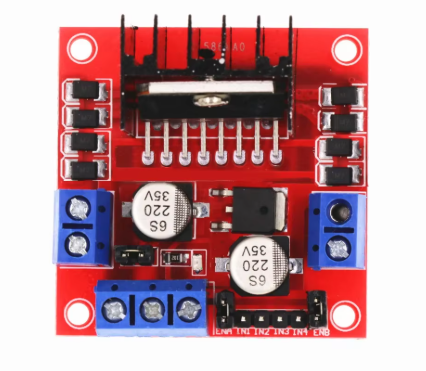
\includegraphics[width=5cm]{figs/control}
  \end{center}
  \caption{Módulo de placa controladora L298N}
  \label{fig:control}
\end{figure}\


\begin{table}[H]
\begin{center}
\begin{tabular}{|c|c|}
\hline
\textbf{Características básicas} & \textbf{Descripción}\\
\hline
Dimensiones & 43mm × 43mm × 27mm \\
\hline
Voltaje lógico & 5V\\
\hline
Corriente lógica & 0mA a 36mA\\
\hline
Peso & 30g\\
\hline
Voltaje de conducción & 5V - 35V\\
\hline
Corriente de conducción & 2A\\
\hline
Almacenamiento & 512 GB SSD\\
\hline
Potencia & 25W \\

\hline
\end{tabular}
\caption{Especificaciones técnicas de controlador L298N}
\label{cuadro:control}
\end{center}
\end{table}


\subsection{Motores}

Para el movimiento del robot se han utilizado dos motores corriente continua (CC)   compatibles con el controlador L298N. Estos motores funcionan con un rango de tensión de 6 a 12V  y permiten el control de velocidad y sentido de giro mediante señales PWM generadas por la Raspberry Pi.

\vspace{0.2cm}


\begin{figure} [h!]
  \begin{center}
    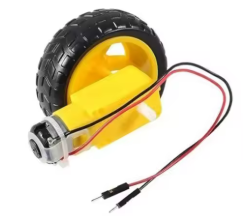
\includegraphics[width=6cm]{figs/rueda}
  \end{center}
  \caption{Motor eléctrico de CC 3-6V}
  \label{fig:rueda}
\end{figure}\


\subsection{Rueda loca}

Para conseguir estabilidad y ayudar en el movimiento del robot se ha incorporado una rueda loca (Figura \ref{fig:loca}). Esta rueda puede girar en todas las direcciones, permitiendo que el robot tenga mayor maniobralidad.

\vspace{0.2cm}

\begin{figure} [h!]
  \begin{center}
    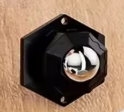
\includegraphics[width=4cm]{figs/loca}
  \end{center}
  \caption{Rueda loca}
  \label{fig:loca}
\end{figure}\


\subsection{Sensor de ultrasonidos}

Para evitar que el robot se acerque demasiado al usuario o al borde de una superficie elevada, se ha utilizado un sensor ultrasonido (Figura \ref{fig:distancia}). Este sensor mide la distancia a los obstáculos mediante la emisión y recepción de ondas ultrasónicas, permitiendo al robot mantener una distancia segura.

\vspace{0.2cm}

\begin{figure} [h!]
  \begin{center}
    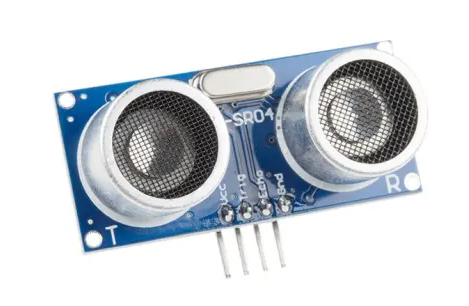
\includegraphics[width=7cm]{figs/distancia}
  \end{center}
  \caption{Sensor de ultrasonidos}
  \label{fig:distancia}
\end{figure}\

\subsection{Pulsador}

Para permitir la interacción con el robot se ha utilizado un pulsador (Figura \ref{fig:boton}). Este botón se conecta directamente a los pines GPIO de la Raspberry Pi.

El pulsador se utiliza como entrada digital, de manera que al ser pulsado genera un señal de activación que es detectada por la Raspberry Pi. En el sistema,  este dispositivo se emplea para iniciar el funcionamiento del robot, facilitando al usuario un control sencillo e intuitivo del sistema.

\vspace{0.2cm}


\begin{figure} [h!]
  \begin{center}
    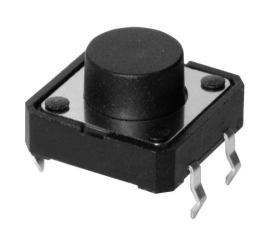
\includegraphics[width=3cm]{figs/boton}
  \end{center}
  \caption{Pulsador}
  \label{fig:boton}
\end{figure}\

\subsection{Router}

Los problemas de conexión a la red pueden provocar fallos en los servicios de cliente-servidor del robot. Para minimizar estos problemas se ha utilizado un router inalámbrico Mercusys AX3000 (Figura \ref{fig:router}).

\vspace{0.2cm}

Este dispositivo permite la creación de una red local en la que se conectan la Raspberry Pi y otros dispositivos del sistema, garantizando una comunicación estable entre los distintos módulos del proyecto.

El router actúa como núcleo de la red, asegurando la conectividad entre los distintos componentes sin depender de una red externa. Las principales especificaciones del router se encuentran descritas en el Cuadro \ref{cuadro:router}.


\vspace{0.2cm}


\begin{figure} [h!]
  \begin{center}
    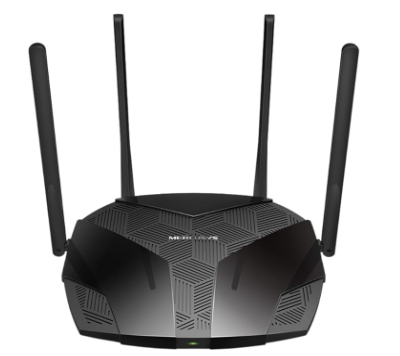
\includegraphics[width=6cm]{figs/router}
  \end{center}
  \caption{MERCUSYS AX3000}
  \label{fig:router}
\end{figure}\


\begin{table}[H]
\begin{center}
\begin{tabular}{|c|c|}
\hline
\textbf{Características básicas} & \textbf{Descripción}\\
\hline
Características del producto & WPS \\
\hline
Clase de banda de frecuencia & 	Banda Doble \\
\hline
Estándar Comunicación Inalámbrica & 802.11ax \\
\hline
Sistema operativo & RouterOS\\
\hline
Ancho de banda del puerto LAN & 1000 Mbps\\
\hline
Número de antenas & 4\\
\hline
Generación del wifi & Wi-Fi 6\\
\hline
Tipo de red del router & dual band \\
\hline
Frecuencia & 160 MHz \\


\hline
\end{tabular}
\caption{Especificaciones técnicas de MERCUSYS AX3000}
\label{cuadro:router}
\end{center}
\end{table}


\subsection{Led}

Un LED (\textit{Light Emitting Diode}) es un componente electrónico semiconductor que emite luz cuando circula corriente a través de él.

Para indicar de forma visual el estado del robot (encendido, apagado o reiniciando) se ha añadido un LED (Figura \ref{fig:led})

\vspace{0.2cm}

\begin{figure} [h!]
  \begin{center}
    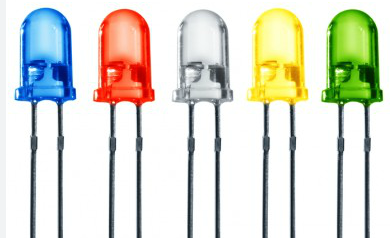
\includegraphics[width=4cm]{figs/led}
  \end{center}
  \caption{LED}
  \label{fig:led}
\end{figure}\


\subsection{Ordenador principal}

En el desarrollo de este proyecto ha sido necesario utilizar un ordenador principal para poder usar algoritmos más complejos que la Raspberry no puede soportar; como por ejemplo, un reconocimiento facial óptimo o el uso de LLM (\textit{Large Language Models}) fluido.
Se ha utilizado un Victus 16-e0xxx (Figura \ref{fig:pc}) cuyas especificaciones se describen en el Cuadro \ref{cuadro:pc}.

\vspace{0.2cm}

\begin{figure} [h!]
  \begin{center}
    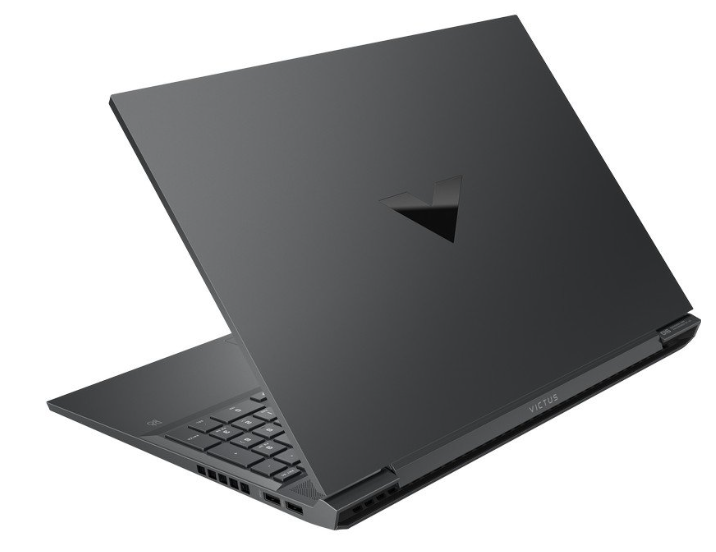
\includegraphics[width=8cm]{figs/pc}
  \end{center}
  \caption{Victus 16-e0xxx}
  \label{fig:pc}
\end{figure}\


\begin{table}[H]
\begin{center}
\begin{tabular}{|c|c|}
\hline
\textbf{Características básicas} & \textbf{Descripción}\\
\hline
Dimensiones & 370 mm × 260 mm × 23.5 mm \\
\hline
Peso & 	2.46 kg \\
\hline
Batería & 70 Wh \\
\hline
Procesador (CPU) & AMD Ryzen 5000 series\\
\hline
Tarjeta gráfica (GPU) & GeForce RTX 3050\\
\hline
Memoria RAM & 16 GB\\
\hline
Almacenamiento & 512 GB SSD\\
\hline
Sistema operativo & Windows 11 y Ubunto 22.4 \\

\hline
\end{tabular}
\caption{Especificaciones técnicas de Victus 16-e0xxx}
\label{cuadro:pc}
\end{center}
\end{table}


\subsection{Impresora 3D Creality}

Para la fabricación de los piezas diseñadas en 3D se ha utilizado la impresora \textit{Creality CR-6 SE} (Figura \ref{fig:impresora}). Esta impresora ofrece una calidad de impresión suficiente para fabricar con precisión piezas que componen la estructura del robot.

\vspace{0.2cm}

\begin{figure} [h!]
  \begin{center}
    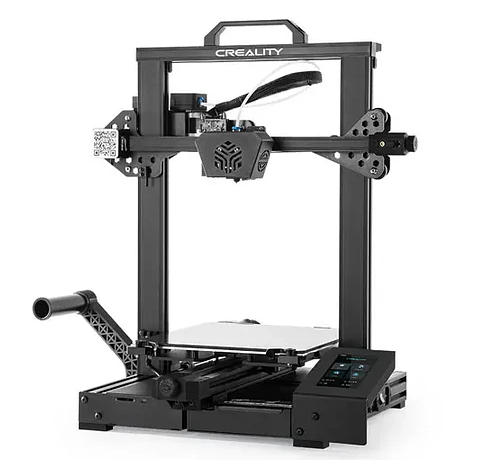
\includegraphics[width=8cm]{figs/impresora}
  \end{center}
  \caption{Impresora Creality CR6 SE}
  \label{fig:impresora}
\end{figure}\



\section{Software}
\label{sec:software}

En está sección se describen las diferentes herramientas software que se han usado para la implementación del proyecto.

\subsection{Sistema operativo}

El sistema operativo seleccionado para la Raspberry ha sido Debian 12, una versión estable y reciente lanzada en 2023. Esta distribución se ha elegido por su alta compatibilidad con la Raspberry Pi y, especialmente, por la versión de Python que incorpora por defecto (Python 3.11), la cual resulta compatible con las librerías utilizadas para el desarrollo del proyecto. Además, permite la ejecución de interfaces gráficas y herramientas necesarias para la interacción del robot.
Se evaluó el uso de Ubuntu 20.04; sin embargo, no disponía de interfaz gráfica para la Raspberry Pi, lo cual constituye un requisito importante en este trabajo.

\vspace{0.2cm}

Por otro lado, el portátil utilizado para el desarrollo cuenta con Ubuntu 22.04 LTS (Long Term Support), una versión estable y ampliamente utilizada en entornos de desarrollo, lo que garantiza compatibilidad y fiabilidad.



\subsection{FreeCAD}

Para el diseño y modelado 3D se ha utilizado la herramienta de código abierto y gratuita FreeCAD (Figura \ref{fig:freecad}).

Esta aplicación permite crear modelos paramétricos tanto en 2D como 3D, facilitando la modificación del diseño mediante el ajuste de dimensiones y restricciones sin la necesidad de rehacer el modelo completo. Su funcionamiento se basa en la creación de  bocetos que posteriormente se transforman en objetos tridimensionales mediante operaciones extrusión o revolución.
Además, cuenta con diversos entornos de trabajo (\textit{workbenches}) que amplían sus funcionalidades en función del tipo de diseño.

\vspace{0.2cm}

Es compatible con diversos formatos de archivo como DAE, DXF o STL, siendo este último el formato más utilizado para la impresión 3D.


\vspace{0.2cm}

\begin{figure} [h!]
  \begin{center}
    
\includegraphics[width=8cm]{figs/freecad}
  \end{center}
  \caption{Logotipo de FreeCAD 1.0}
  \label{fig:freecad}
\end{figure}\


\subsection{Python}

Python es un lenguaje de programación de alto nivel, interpretado y orientado a objetos, ampliamente utilizado en la comunidad de programadores debido a su sencillez y legibilidad.
Al tratarse de un lenguaje interpretado, el código es ejecutado mediante un intérprete en tiempo de ejecución, lo que facilita su desarrollo, prueba y depuración.

\vspace{0.2cm}

Python cuenta con una amplia biblioteca estándar y un ecosistema de bibliotecas externas, lo que permite el desarrollo de múltiples tipos de aplicaciones, como aprendizaje automático (TensorFlow, Pandas, PyTorch), o computación científica (math, NumPy), entre otras.

\vspace{0.2cm}

Debido a su versatilidad y facilidad de uso, este lenguaje ha sido seleccionado para implementar el código.


\subsection{OpenCV}

OpenCV\footnote{https://opencv.org/} (Figura \ref{fig:opencv}) es una biblioteca libre y de código abierto diseñada para visión artificial y procesamiento de imágenes.

Fue desarrollada por Intel en 1999 y, desde entonces, se ha consolidado en una de las herramientas más utilizadas y robustas del campo de visión por computador.

\vspace{0.2cm}

Esta biblioteca permite realizar tareas como la captura, procesamiento y análisis de imágenes, incluyendo la detección de objetos y tratamiento de vídeo en tiempo real.

En este proyecto se ha utilizado OpenCV para capturar de imágenes y su envío  al servidor para su procesamiento.

\vspace{0.2cm}

\begin{figure} [h!]
  \begin{center}
    
\includegraphics[width=4cm]{figs/opencv}
  \end{center}
  \caption{Logotipo de FreeCAD 1.0}
  \label{fig:opencv}
\end{figure}\


\subsection{LLM}

Los modelos LLM son modelos de aprendizaje profundo entrenados con grandes volúmenes de datos, capaces de comprender, procesar y generar lenguaje natural.

\vspace{0.2cm}

Una de las funcionalidades del sistema incluye el reconocimiento por voz y procesamiento del lenguaje natural, con el objetivo de conseguir una interacción humano-robot más fluida. En este contexto, se han evaluado distintos modelos, recogidos en el Cuadro \ref{cuadro:llm}, con el fin de analizar su rendimiento y seleccionar el más adecuado para su integración en el sistema.

\begin{table}[H]
\centering
\small
\begin{tabularx}{\textwidth}{|c|c|X|c|X|}
\hline
\textbf{Modelo} &
\makecell{\textbf{Latencia}\\\textbf{media (s)}} &
\makecell{\textbf{Tipo de}\\\textbf{ejecución}} &
\textbf{Coste} &
\makecell{\textbf{Calidad de}\\\textbf{respuesta}} \\
\hline
LLaMA 2 7B & 33.8 & Local & Hardware & 2/5 \\
\hline
LLaMA 3.3 70B & 2.4 & API & Freemium & 3/5 \\
\hline
Mistral 7B & 30.0 & Local & Hardware & 2/5 \\
\hline
Gemini Flash Latest & 15.2 & API & Pago por tokens & 4/5 \\
\hline
GPT-4o Mini & 3.7 & API & Pago por tokens & 4/5 \\
\hline
\end{tabularx}
\caption{Comparativa LLMs}
\label{cuadro:llm}
\end{table}


\vspace{0.2cm}


Finalmente, se ha seleccionado LlaMA 3.3 70B en su variante Versatile, ejecutado mediante el motor de inferencia Groq, debido a que presenta el mejor compromiso entre latencia y calidad de respuesta, cumpliendo los requisitos del sistema en términos de rendimiento y coste.



\subsection{Bibliotecas externas}

Además de las herramientas anteriormente descritas, se han utilizado otras de propósito general. Por otro lado, la biblioteca \verb|face_recognition| se ha utilizado para la detección  y reconocimiento facial en imágenes. Para la comunicación cliente-servidor se ha empleado \verb|base64| para la codificación y envío de imágenes, \verb|flask| para el desarrollo de una API encargada de gestionar rutas URL y manejar las solicitudes HTTP (GET y POST), y \verb|requests| para realizar peticiones al servidor.


Por otro lado, para el almacenamiento de los rostros reconocidos se ha utilizado la biblioteca \verb|pickle|. Para la creación de la interfaz gráfica se ha empleado \verb|PyQt5|, mientras que el desarrollo de los juegos interactivos se ha realizado con \verb|pygame|.

Para el uso del LCD se han utilizado las bibliotecas \verb|adafruit_rgb_display|, \verb|digitalio|, \verb|busio| y \verb|board|.

Finalmente para la reproducción de audio se ha utilizado \verb|vosk|.


